\chapter{Arquitetura Básica do RouteFlow}

\section{Descrição do Protocolo Openflow}

O \textit{OpenFlow} foi proposto pela Universidade de Stanford para atender à demanda de validação
de novas propostas de arquiteturas e protocolos de rede (incluindo as abordagens \textit{clean slate})
sobre equipamentos comerciais. O \textit{OpenFlow} define um protocolo-padrão para determinar as
ações de encaminhamento de pacotes em dispositivos de rede, como, por exemplo,
comutadores, roteadores e pontos de acesso sem fio. As regras e ações instaladas no
hardware de rede são responsabilidade de um elemento externo, denominado controlador, que
pode ser implementado em um servidor comum, conforme Figura \ref{fig:openflow}. 

\begin{figure}[hb]
\centering
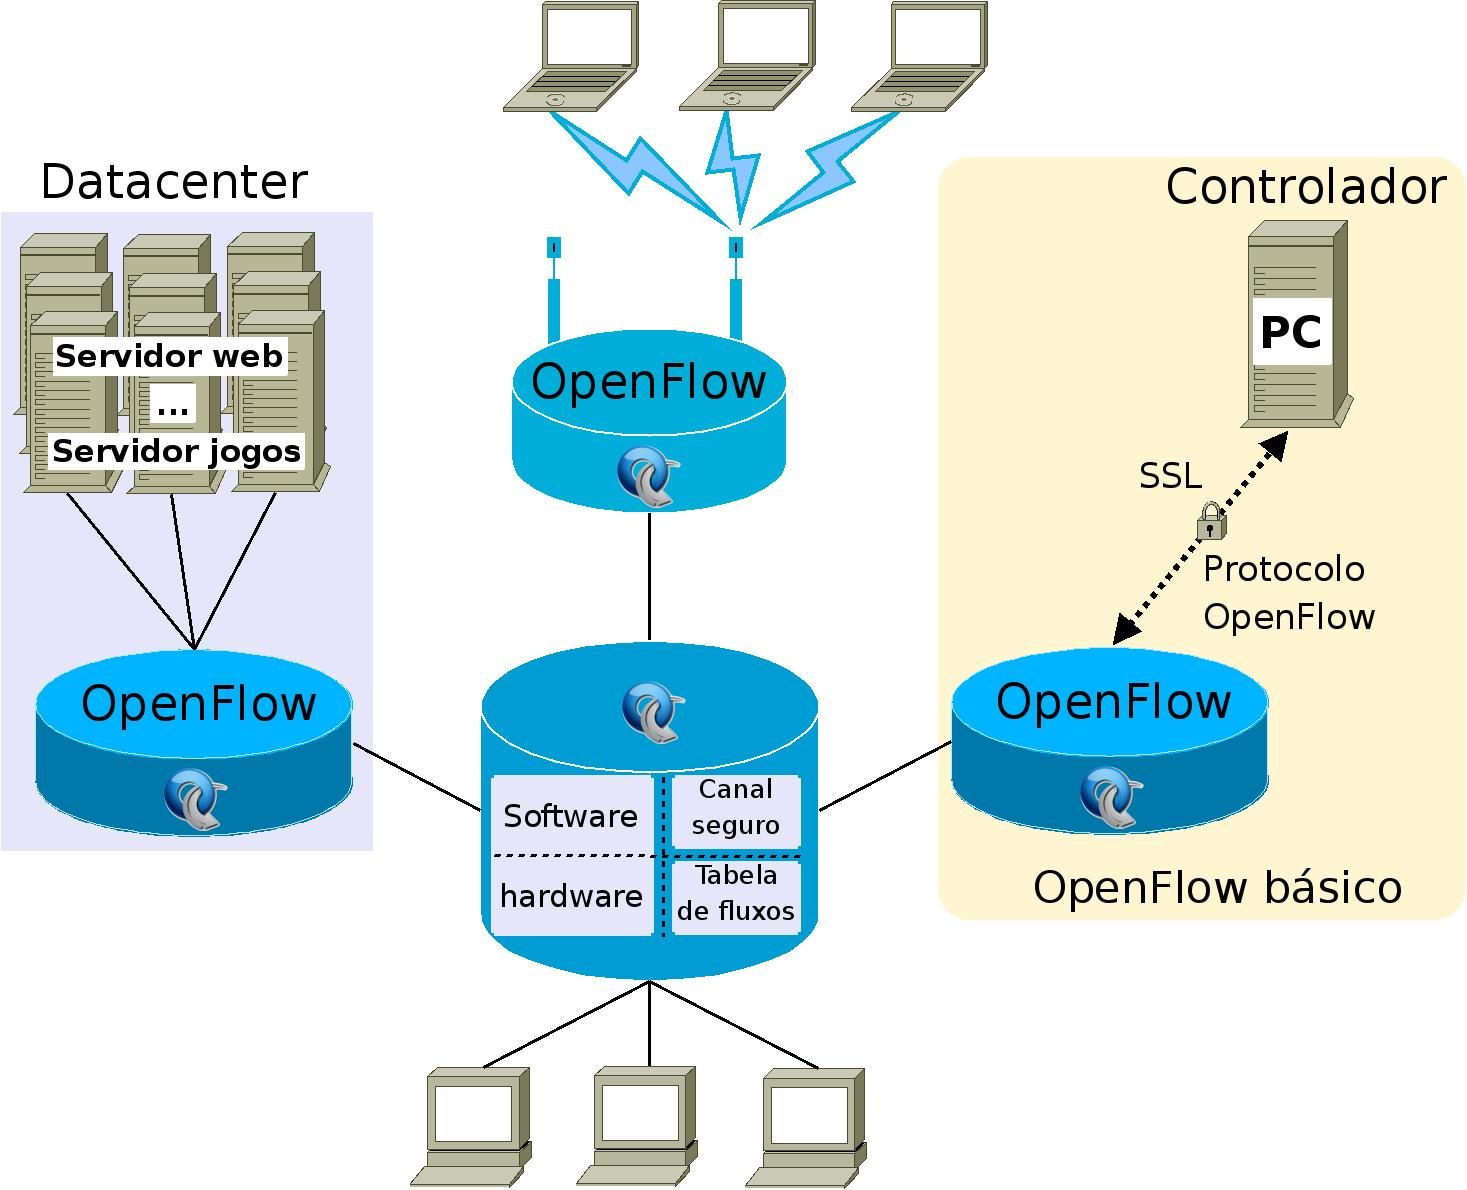
\includegraphics[width=110mm]{openflow.png}
\caption{Rede com OpenFlow Habilitado}
\label{fig:openflow}
\end{figure}

A principal abstração utilizada na especificação \textit{OpenFlow} é o conceito de fluxo. Um fluxo é
constituído pela combinação de campos do cabeçalho do pacote a ser processado pelo
dispositivo, conforme Figura \ref{fig:cabecalhoOpenflow}. As tuplas podem ser formadas por campos das camadas de
enlace, de rede ou de transporte, segundo o modelo \textit{TCP/IP}. Deve-se enfatizar que a
abstração da tabela de fluxos ainda está sujeita a refinamentos, com o objetivo de oferecer uma
melhor exposição dos recursos do hardware e, nesse caso, permitir a concatenação de várias
tabelas já disponíveis, como, por exemplo, tabelas \textit{IP/Ethernet/MPLS}. Nesse sentido, a
contribuição mais importante do paradigma do \textit{OpenFlow} é a generalização do plano de dados –
qualquer modelo de encaminhamento de dados baseado na tomada de decisão fundamentada
em algum valor, ou combinação de valores, dos campos de cabeçalho dos pacotes pode ser
suportado. 

\begin{figure}[hb]
\centering
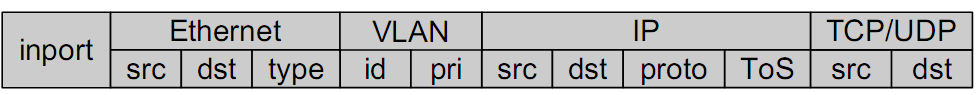
\includegraphics[width=160mm]{cabecalhoOpenflow.png}
\caption{Cabeçalho OpenFlow para a especificação dos fluxos}
\label{fig:cabecalhoOpenflow}
\end{figure}

De forma pragmática, a especificação \textit{OpenFlow} (OPENFLOW, 2010) procura reutilizar as
funcionalidades do hardware existente (por exemplo, Access Control List – ACL em switches
e roteadores para implementar serviços como NAT, firewall e VLANs) através da definição de
um conjunto simples de regras e das ações associadas: encaminhar, descartar, enviar para o
controlador, reescrever campos do cabeçalho, etc. 

\section{Introdução ao RouteFlow}

O RouteFlow é uma proposta de oferta de serviços de roteamento IP remoto de forma
centralizada, e que visa um desacoplamento efetivo entre o plano de encaminhamento e o
plano de controle (ROUTEFLOW, 2011). O objetivo é tornar as redes IP mais flexíveis pela
facilidade de adição, remoção e especialização de protocolos e algoritmos. O RouteFlow
armazena a lógica de controle dos switches OpenFlow na infraestrutura de rede, através de
uma rede virtual composta por máquinas virtuais (MV), cada uma executando um código (engine)
de roteamento de domínio público (open source). Essas MVs podem ser interconectadas de
maneira a formar uma topologia lógica, espelhando a topologia de uma rede física
correspondente ou uma topologia virtual simplificada. O ambiente virtual é armazenado
em um servidor externo, ou um conjunto deles, que se comunicam com os equipamentos do
plano de dados através de um controlador OpenFlow, que transporta para o plano de
encaminhamento as decisões tomadas pelos protocolos de roteamento no plano de controle
(OSPF, BGP, RIP). A Figura \ref{fig:visaoGeralRouteFlow} ilustra uma sub-rede com switches programáveis, em que a
lógica de roteamento é implementada no servidor RouteFlow. 
O resultado consiste numa solução flexível de alto desempenho e comercialmente competitiva,
a partir da combinação de recursos disponíveis, como, por exemplo:

\begin{enumerate}[{a)}]
\item switches programáveis de baixo custo e software embarcado reduzido (OpenFlow); 
\item pilhas de protocolos de roteamento open source (QUAGGA, 2009; XORP, 2011); e 
\item servidor de prateleira de alto poder de processamento e, também, de baixo custo.
\end{enumerate}

Cabe ressaltar que, apesar de o controle estar fisicamente centralizado, ele continua distribuído
logicamente. Dessa forma, não é necessária qualquer alteração dos protocolos de roteamento
existentes. Além disso, a solução pode tornar-se mais escalável no futuro, com o uso de vários
servidores de alto desempenho.

\begin{figure}[hb]
\centering
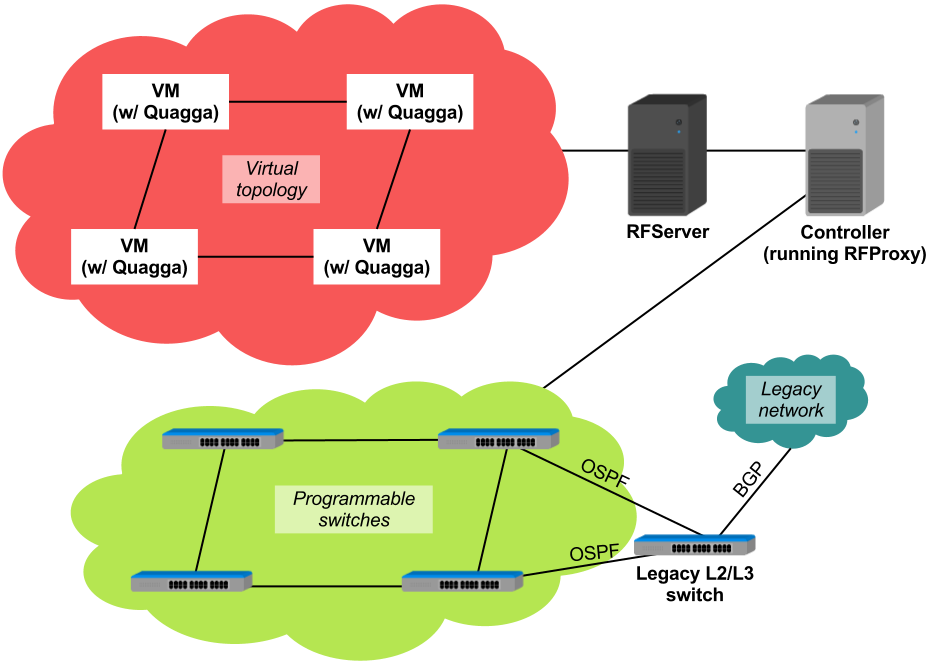
\includegraphics[width=135mm]{visaoGeralRouteFlow.png}
\caption{Visão geral do RouteFlow}
\label{fig:visaoGeralRouteFlow}
\end{figure}

\section{Descrições dos Principais Componentes do RouteFlow}

O RouteFlow é dividido basicamente em três aplicações básicas: RFClient, RFServer e RFProxy. Na Figura \ref{fig:componentesRouteFlow} temos uma visão geral das aplicações:

\begin{itemize}
\item RFClient executa como um programa executável em um máquina virtual, detectando mudanças na tabela ARP do Linux e na tabela de roteamento. As informações de roteamento são enviadas para o RFServer quando são atualizadas.

\item RFServer é uma aplicação independente que gerencia as máquinas virtuais que estão executando o RFClient. O RFServer mantem o mapeamento entre as instâncias das máquinas virtuais executando o RFClient e as interfaces correspondentes aos switches e suas respectivas portas. É conectado ao RFProxy para instruí-lo como configurar os fluxos e também como configurar o Open vSwitch que mantém a conectividade de todo o ambiente composto pelas máquinas virtuais.

\item RFProxy é uma aplicação responsável pelas interações entre os switches OpenFlow (identificados pelos seus datapaths) via o protocolo OpenFlow. Ele aguarda instruções do RFServer e o notifica à respeito de eventos na rede. Atualmente é executado como um módulo vinculado aos controladores OpenFlow. O RouteFlow tem suporte aos controladores NOX e POX, sendo que a proposta do trabalho é adicionar suporte ao Floodlight.
\end{itemize}

\begin{figure}[hb]
\centering
\includegraphics[width=125mm]{componentesRouteFlow.png}
\caption{Componentes principais do RouteFlow}
\label{fig:componentesRouteFlow}
\end{figure}

\section{Protocolo RouteFlow}

É o protocolo desenvolvido e usado para a comunicação entre os componentes do RouteFlow. Nele, estão definidas as mensagens e os comandos básicos para conexão e
configuração das máquinas virtuais e, também, gerenciamento das entradas de roteamento em hardware. Entre os campos da mensagem-padrão estão: identificação do controlador,
identificação da máquina virtual, tipo da mensagem, comprimento e dados. O proxy RouteFlow recebe os  comandos do servidor RouteFlow através deste protocolo e de acordo com o tipo de comando executa as principais ações, muitas delas exigindo a comunicação com os switches físicos. A comunicação com os switches físicos é feita via protocolo OpenFlow, fazendo o proxy RouteFlow agir como uma espécie de "tradutor" entre os dois protocolos.